% Created 2015-02-19 Thu 23:09
\documentclass[11pt]{article}
\usepackage[utf8]{inputenc}
\usepackage[T1]{fontenc}
\usepackage{fixltx2e}
\usepackage{graphicx}
\usepackage{longtable}
\usepackage{float}
\usepackage{wrapfig}
\usepackage{soul}
\usepackage{textcomp}
\usepackage{marvosym}
\usepackage{wasysym}
\usepackage{latexsym}
\usepackage{amssymb}
\usepackage{hyperref}
\tolerance=1000
\usepackage{methodshw, amsmath}
\usepackage{booktabs}
\providecommand{\alert}[1]{\textbf{#1}}

\title{8004 Homework 4}
\author{Nooreen Dabbish}
\date{\today}
\hypersetup{
  pdfkeywords={},
  pdfsubject={},
  pdfcreator={Emacs Org-mode version 7.9.3f}}

\begin{document}

\maketitle




\section{Problem 1 In the context of Problem 2 of Homework Assignment 3, use R matrix calculations to do the following in the (non-full-rank) Gauss-Markov normal linear model}
\label{sec-1}
\subsection{Find 90\% two-sided confidence limits for $\sigma$.}
\label{sec-1-1}


The model described in HW3, Problem 2 in 
$\mathbf{Y}=\mathbf{X\beta}+\epsilon$ matrix form is:

\[
\begin{pmatrix}
y_{11} \\ y_{12}\\ y_{21}\\ y_{31}\\ y_{41}\\ y_{42}
\end{pmatrix} = 
\begin{pmatrix} 
2\\ 1\\ 4\\ 6\\ 3\\ 5
\end{pmatrix} = 
\begin{pmatrix}
1 & 1 & 0 & 0 & 0 \\
1 & 1 & 0 & 0 & 0 \\
1 & 0 & 1 & 0 & 0 \\
1 & 0 & 0 & 1 & 0 \\
1 & 0 & 0 & 0 & 1 \\
1 & 0 & 0 & 0 & 1 \\
\end{pmatrix}  
\begin{pmatrix}
\mu \\ \tau_1 \\ \tau_2 \\ \tau_3 \\ \tau_4 
\end{pmatrix} + 
\begin{pmatrix}
\epsilon_{11} \\ \epsilon_{12}\\ \epsilon_{21}\\ \epsilon_{31}\\ \epsilon_{41}\\ \epsilon_{42}
\end{pmatrix}
\]

Because the problem statement says this is a Gauss-Markov normal
linear model, we know that \textbf{Y} $\sim$ N(\textbf{X$\beta$},$\sigma$$^2$ \textbf{I}).
\subsubsection{SSE/$\sigma$$^2$}
\label{sec-1-1-1}


Using theorem 1 in the Appendix, we can show:

$$\frac{SSE}{\sigma^2} = \frac{(\mathbf{Y} -
\hat{\mathbf{Y}})'(\mathbf{Y} - \hat{\mathbf{Y}})}{\sigma^2} \sim
\chi^2_{n-\text{rank}(X)}$$

Rearranging to find confidence limits for $\sigma$ gives:

$$P\left(\sqrt{\frac{SSE}{\mathrm{upper\, \alpha/2\, quantile\, of\,
\chi^2_{n-\mathrm{rank}(X)}}}} < \sigma < \sqrt{\frac{SSE}{\mathrm{upper\, \alpha/2\, quantile\, of\, \chi^2_{n-\mathrm{rank}(X)}}}} \right)
= 1 - \alpha$$
\subsubsection{Solution from R}
\label{sec-1-1-2}

Using the hand-written function \verb~sigmacalc~, included in the
appendix. The following two-sided 90\% confidence limits for $\sigma$ 
were obtained: \texttt{0.646} <
$\sigma$ < \texttt{4.9366}.
\subsection{Find 90\% two-sided confidence limits for $\mu$ + $\tau$$_2$.}
\label{sec-1-2}


Using the t-distribution describing the distribution of estimable
function c'$\beta$, the handwritten R function \verb~cbetacalc~ included in
the appendix, was used to caluclate confidence limits for this
entity, where c' = (1, 0, 1, 0 , 0).

\texttt{0.7354} 
< $\mu$ + $\tau$$_2$ <
\texttt{7.2646}
\subsubsection{Estimable functions \textbf{c'$\beta$}}
\label{sec-1-2-1}


For an estimable \textbf{c'$\beta$}, we have:

$$\frac{\widehat{\mathbf{c'\beta}} -
\mathbf{c'\beta}}{\sqrt{MSE}\sqrt{\mathbf{C'(X'X)^{-}C}}} \sim
t_{n-\mathrm{rank}(X)}$$

Note that $MSE = \frac{SSE}{n-\mathrm{rank}(X)}$. Rearranging to find 1 - $\alpha$ confidence limits for \textbf{c'$\beta$},
denoting t$^{\star}$ = the upper $\alpha$/2 quantile of t$_{\mathrm{n-rank(X)}}$, we
have:

$$P\left( \widehat{\mathbf{c'\beta}} -
t^{\star}\sqrt{MSE}\sqrt{\mathbf{C'(X'X)^{-}C}} < \mathbf{c'\beta} <  \widehat{\mathbf{c'\beta}} +
t^{\star}\sqrt{MSE}\sqrt{\mathbf{C'(X'X)^{-}C}} \right) = 1 - \alpha$$
\subsection{Find 90\% two-sided confidence limits for $\tau$$_1$ - $\tau$$_2$.}
\label{sec-1-3}
\label{Tau1Tau2}

Proceeding as in \hyperref[MuTau2]{part b}, here $\tau$$_1$ - $\tau$$_2$ = \textbf{c}'\textbf{$\beta$} = $(0, 1, -1,
0, 0) \begin{pmatrix} \mu \\ \tau_1 \\ \tau_2
\\ \tau_3 \\ \tau_4 \end{pmatrix}$. The function \verb~cbetacalc~ was used
once again with \textbf{c} above. 

\texttt{-6.4984} 
< $\tau$$_1$ - $\tau$$_2$ <
\texttt{1.4984}
\subsection{Find a \emph{p}-value for testing the null hypothesis $H_0 : \tau_1 - \tau_2 = 0$ vs \emph{H$_a$} : not \emph{H$_0$}.}
\label{sec-1-4}
\subsubsection{General Linear Hypothesis Test}
\label{sec-1-4-1}

\emph{The general linear hypothesis test} is the following F test for
\emph{H$_0$} : \textbf{C$\beta$} = \textbf{0} verus \emph{H$_1$} : \textbf{C$\beta$} $\neq$ \textbf{0}, given \textbf{y}
$\sim$ N$_n$(\textbf{X$\beta$},$\sigma$$^2$ \textbf{I}), \textbf{C} \emph{q} x (/k/+1), rank(\textbf{C}) = q, with SSH = the sum of squares due to
the hypothesis or due to \textbf{C$\beta$}. Note that 

\(\frac{SSH}{\sigma^2} = \frac{(\mathbf{C\hat{\beta}})'[\mathbf{C(X'X)^{-1}C}']^{-1}\mathbf{C\hat{\beta}}}{\sigma^2}
\sim
\chi^2(q,\frac{(\mathbf{C\beta})'[\mathbf{C(X'X)^{-1}C}']^{-1}\mathbf{C\beta}}{2\sigma^2})\)

\noindent and

\(\frac{SSE}{\sigma^2} = \frac{\mathbf{y}'[\mathbf{I} -
\mathbf{X(X'X)^{-1}X}']\mathbf{y}}{\sigma^2} \sim \chi^2(n-rank(X)).\)

Taking the ratio gives us our test statistic:
$$F = \frac{SSH/q}{SSE/(n-rank(X))}$$

\begin{itemize}
\item If \emph{H$_0$} : \textbf{C$\beta$} = \textbf{0} is false, F $\sim$ F(q,n-rank(X),$\lambda$), where
  $\lambda =
  \frac{(\mathbf{C\beta})'[\mathbf{C(X'X)^{-1}C}']^{-1}\mathbf{C\beta}}{2\sigma^2})$.
\item Notice that if \textbf{C$\beta$} = \textbf{0} is true, $\lambda$ defined above = 0, giving F
  $\sim$ F(q, n-rank(X)).
\end{itemize}
\subsubsection{\emph{p}-value from the F statistic}
\label{sec-1-4-2}


We need to find the F statistic described above. Here \textbf{C} is \textbf{a}' from
\hyperref[Tau1Tau2]{above}, \textbf{a}'=(0,1,-1,0,0), and \textbf{C} is 1 x 5, rank 1.

We used the handwritten function \verb~Cbetahatd~ throughout for
General Linear Hypothesis Testing. It is included in the appendix for
your reference.

The \emph{p}-value obtained was \texttt{0.209430584957905}. 
\subsection{Find 90\% two-sided predition limits for the sample mean of \emph{n} = 10 future observations from the first set of conditions.}
\label{sec-1-5}
\subsubsection{A t statistic for prediction}
\label{sec-1-5-1}


Consider future observation y$_0$, y$_0$ = \textbf{x$_0$}' $\beta$ + $\epsilon$$_0$ with
$\hat{y}_0 = \mathbf{x_0'\hat{\beta}}$, where $\hat{y_0}$ is computed
from \emph{n} observations and y$_0$ is obtained independently. We find that
$E(y_0 - \hat{y_0}) = 0$ and 


$var(y_0 - \hat{y}_0) = var(\epsilon_0) +
var(\mathbf{x_0'\hat{\beta}}) = \sigma^2[1+
\mathbf{x_0'(X'X)^{-1}x_0}]$, where 
$\widehat{var(y - \hat{y}_0)} = s^22[1+ \mathbf{x_0'(X'X)^{-1}x_0}]$. Because of the independence of \emph{s$^2$}
and \emph{y$_0$} and $\hat{y}_0$, we have the following t statistic:

$$t = \frac{y_0 - \hat{y}_0 - 0}{s\sqrt{1+
\mathbf{x_0'(X'X)^{-1}x_0}}} \sim t(n-\mathrm{rank}(X))$$



Therefore,

$$P = \left[ -t_{\alpha/2,n-rank(X)} \leq \frac{y_0 - \hat{y}_0 - 0}{s\sqrt{1+
\mathbf{x_0'(X'X)^{-1}x_0}}} \leq t_{alpha/2,n-rank(X)}\right] = 1 -
\alpha$$

Re-arranging in terms of $\mathbf{x_0'\hat{\beta}} = \hat{y}_0$ gives:

$$\mathbf{x_0'\hat{\beta}} \pm t_{\alpha/2,n-rank(X)}s\sqrt{1+
\mathbf{x_0'(X'X)^{-1}x_0}}.$$
\subsubsection{Predicitions for \emph{n} observations from $\mu$ + $\tau$$_1$}
\label{sec-1-5-2}


Using the preceeding theory and the handwritten R function,
\verb~predict~, which is included in the appendix. I ran a prediction fo
\emph{n} =10 from the first condition  \textbf{x$_0$} = (1,1,0,0,0).

The 90\% confidence limits obtained for the mean were 
\texttt{-1.0288} 
to
\texttt{4.0288}.
\subsection{Find 90\% two-sided prediction limits for the difference between a pair of future values, one from the first set of conditions (i.e. with mean $\mu$ + $\tau$$_1$) and one from the second set of conditions (i.e. with mean $\mu$ + $\tau$$_2$).}
\label{sec-1-6}


Similar to part (e) above, here I used my \verb~predict~ function again,
except an \emph{n} of .5 in order to obtain a gamma of 2 and a \textbf{x$_0$} vector of the 
difference of the first two conditions:

(1,1,0,0,0) - (1,0,1,0,0) = (0,1,-1,0,0).

This gave 90 \% prediction limits for the difference as follows:
\texttt{-8.6076}
to
\texttt{3.6076}.
\subsection{Find a \emph{p}-value for testing the following: What is the practical interpretation of this test?}
\label{sec-1-7}

\( H_0 : \begin{pmatrix} 0 & 1 & -1 & 0 & 0 \\ 0 & 1 & 0 & -1 & 0 \\ 0 & 1 & 0 & 0 & -1 \end{pmatrix} \begin{pmatrix} \mu \\ \tau_1 \\ \tau_2 \\ \tau_3 \\ \tau_4 \end{pmatrix} = \begin{pmatrix} 0 \\ 0 \\ 0 \end{pmatrix}. \) 

The null hypothesis asked by this test is whether $\tau$$_1$ = $\tau$$_2$ =
tau$_3$ = tau$_4$, if all these parameters are equal there would be no
difference among the treatments. I performed the test using the General Linear
Hypothesis Testing function described above, \verb~Cbetahatd~, with the
matrix above as C in C'$\beta$ and the d-vector = (0,0,0).


\begin{verbatim}
G <- t(matrix(c(0,1,-1,0,0,
                      0,1,0,-1,0,
                      0,1,0,0,-1),nrow=3,ncol=5, byrow=TRUE))
    Cbetahatd(Y1,X1,G,c(0,0,0))
\end{verbatim}


I obtained a p value of 0.20643991448067, indicating that it is
unlikely that all of the parameters are equal. 
\subsection{Find a \emph{p}-value for testing:}
\label{sec-1-8}

\(H_0 : \begin{pmatrix} 0 & 1 & -1 & 0 & 0 \\ 0 & 0 & 1 & -1 & 0
\end{pmatrix} \begin{pmatrix} \mu \\ \tau_1 \\ \tau_2 \\ \tau_3
\\ \tau_4 \end{pmatrix} = \begin{pmatrix} 10 \\ 0  \end{pmatrix}.\)

In this test, the null hypothesis asks whether $\tau$$_1$ - $\tau$$_2$ = 10
and $\tau$$_2$ = $\tau$$_3$. I tested this hypotheis as in question 1g), using the General Linear
Hypothesis and the F-test implemented in my function \verb~Cbetahatd~,
note that the vector (10,0) was entered for the \textbf{d} vector.


\begin{verbatim}
H <- t(matrix(c(0, 1, -1, 0, 0, 0, 0, 1, -1, 0), nrow=2, ncol=5, byrow=T))

   Cbetahatd(Y1,X1,H,c(10,0))
\end{verbatim}

A significant \emph{p}-value of 0.0134 was obtained, suggesting that this
hypothesis is acceptable.
\section{Problem 2 In the following make use of the data in Problem 4 of Homework Assignment 3. Consider a regression of \emph{y} on $x_1, x_2,\ldots,x_5$. Use R matrix calculations to do the following in a full rank Gauss-Markov normal linear model.}
\label{sec-2}
\subsection{Find 90\% two-sided condifence limits for $\sigma$.}
\label{sec-2-1}


Calling our \verb~sigmacalc~ function on the Boston data set, we find 90\%
confidence limits for sigma of
\texttt{5.6106} < $\sigma$ < \texttt{6.2263}.
\subsection{Find 90\% two-sided confidence limits for the mean response under the conditions of data point \#1.}
\label{sec-2-2}



To find these 90\% confidence limits, we will use the t$_{\mathrm{n-rank(X)}}$-distribution
of $\frac{\widehat{c'\beta} -
c'\beta}{\sqrt{MSE}{\sqrt{c'(X'X)^{-}c}}$, 
where c' is the first row of our data set
(data point \#1).

Using the \verb~cbetacalc~ function to do this, as \verb~cbetacalc(YB,XB, .1, XB[1,])~ we find a 90\% confidence interval for the mean response under the
conditions of data point \#1 of 
\texttt{25.2114} 
to 
\texttt{26.1973}.
\subsection{Find 90\% two-sided condifence limits for the difference in mean responses under the conditions of data points \#1 and \#2. .}
\label{sec-2-3}



To find these 90\% confidence limits, we will use the t-distribution
function of c'$\beta$ again, where c' is the difference beteen the first row
of our data set and the second row
(data points \#1 and \#2).

Using the \verb~cbetacalc~ function to do this, as \verb~cbetacalc(YB,XB, .1, (XB[1,]-XB[2,]))~ we find \texttt{1.2025} 
to \texttt{2.6125} is a 90\% confidence interval for the
difference in mean responses under conditions 1 and 2.
\subsection{Find a \emph{p}-value for testing the hypothesis that the conditions of data points \#1 and \#2 produce the same mean response.}
\label{sec-2-4}


An F-test was used to test the hypothesis that the product between the vector describing
the differences between conditions 1 and 2 and beta is \textbf{0}. That is
\emph{H$_0$} : c'$\beta$ = \textbf{0}, where c' = XB[1,] - XB[2,]. This was done using
my general linear hypothesis testing function: \verb~Cbetahatd(YB,XB, (XB[1,]-XB[2,]))~. The \emph{p}-value obtained was \texttt{1.01975837067947e-05}.
\subsection{Find 90\% two-sided prediction limits for an additional response for the set of conditions x$_1$ = 0.005, x$_2$ = 0.45, x$_3$ = 7, x$_4$ = 45, and x$_5$ = 6.}
\label{sec-2-5}


90 \% prediction limits for an additional response from these
conditions were obtained using the conditions as our c-vector in the
\verb~predict~ function: \verb~predict(YB,XB, .1, c(1,0.005,0.45,7,45,6), 1)~ .
The limits obtained were 
\texttt{19.9002} to
\texttt{39.4029}.
\subsection{Find a \emph{p}-value for testing the hypothesis that a model including only \emph{x$_1$}, \emph{x$_3$}, and \emph{x$_5$} is adequare for ``explaining'' home price.}
\label{sec-2-6}


 We use an F-test implementation of the General Linear Hypothesis
 test using the \verb~Cbetahatd~ function described previously. We are
 testing the hypothesis that $\beta$$_2$ = $\beta$$_4$ =
 0, with a $\mathbf{C} = \begin{pmatrix} 0 & 0 & 1 & 0 & 0 & 0\\ 0 & 0 & 0 & 0
 & 1 & 0\end{pmatrix}$.


To investigate this solution, we also 

\begin{verbatim}

CB <- t(matrix(c(0,0,1,0,0,0,0,0,0,0,1,0),nrow=2,ncol=6,byrow=T))

Cbetahatd(YB,XB,CB)
\end{verbatim}


 This gives a p-value of 3.1907809727727e-13, heavily supporting the
 reduced model.
\subsubsection{Full--Reduced model approach}
\label{sec-2-6-1}

We can create a \emph{p}-value to test these models using an F statistic,
constructed out of the ratio of the difference in regression sum of
squares between the full (SSR$_{\mathrm{full}}$) and reduced(SSR$_{\mathrm{reduced}}$) models and the sum of squared
error (SSE). These quantities are independent and follow a
non-central $\chi$$^2$(\emph{h},$\lambda$) and central $\chi$$^2$(\emph{n-k-1})
respectively where \emph{n} is the number of observations, \emph{k} is the
number of parameters in the full model, and \emph{h} is the difference in the
number of parameters between the full and reduced models. The
non-centrality parameter $\lambda$ can be written \textbf{$\beta$$_2$'[X$_2$'X$_2$ - X$_2$'X$_1$(X$_1$'X$_1$)$^{\mathrm{-1}}$X$_1$'X$_2$]$\beta$$_2$/2$\sigma$$^2$} where \textbf{X$_1$} and \textbf{X$_2$}
form a partition of \textbf{X} such that we can write: $$\mathbf{y} =
\mathbf{X\beta} + \mathbf{\epsilon} =
(\mathbf{X}_1,\mathbf{X}_2)\begin{pmatrix} \mathbf{\beta}_1
\\ \mathbf{\beta}_2 \end{pmatrix} + \mathbf{\epsilon} =
\mathbf{X}_1\mathbf{\beta}_1 + \mathbf{X}_2\mathbf{\beta}_2 +
\mathbf{\epsilon} $$

And the reduced model would be \textbf{y} = \textbf{X$_1$$\beta$$_1$$^{\star}$} + $\epsilon$$^{\star}$.



\begin{verbatim}
#Find SSR in the full model.
bhat_B <- ginv(t(XB)%*%XB)%*%t(XB)%*%YB
SSR_Bf <- t(bhat_B) %*% t(XB) %*% YB - (length(YB)*(mean(YB))^2)

#create reduced model design matric and X1_B and estimator bhat1_B
X1_B <- XB[,-c(3,5)]
bhat1_B <- ginv(t(X1_B)%*%X1_B) %*% t(X1_B) %*% YB
SSR_Br <- t(bhat1_B) %*% t(X1_B) %*% YB - (length(YB)*(mean(YB))^2)

YhatB <- XB%*%bhat_B
SSE_B <- t(YB -YhatB)%*%(YB-YhatB)

F_2f <- ((SSR_Bf - SSR_Br)/2)/(SSE_B/(length(YB) - qr(XB)$rank))

pf_2f <- pf(F_2f, 2, (length(YB)-(qr(XB)$rank)), lower.tail=FALSE)
\end{verbatim}

This strategy arrives at a very similar \emph{p}-value: 
\texttt{3.19090353910838e-13}.






 
\section{Problem 3}
\label{sec-3}
\subsection{In the context of Problem 1, part g), suppose that in fact $\tau$$_1$ = $\tau$$_2$, $\tau$$_3$ = $\tau$$_4$ = $\tau$$_1$ - d$\sigma$. What is the distribution of the F statistic?}
\label{sec-3-1}


The F statistic for Problem 1, part g is given by $F =
\frac{Q/s}{SSE/N-\mathrm{rank}(X)} \sim F(s, N-\mathrm{rank}(X),
\lambda)$. 

Where $Q = (\widehat{C'\beta} -
d)'(C'(X'X)^{-}C)^{-1}(\widehat{C'\beta} -d})$ and 
$\lambda = \frac{1}{\sigma^2}(C'\beta -
d)'(C'(X'X)^{-}C)^{-1}(C'\beta -d)$. 

Therefore,
if $\tau$$_1$ = $\tau$$_2$, and $\tau$$_3$=$\tau$$_4$=$\tau$$_1$ - d$\sigma$, our
non-centrality parameter will equal 
$$\lambda = \frac{1}{\sigma^2}(0, d\sigma, d\sigma)
(C'(X'X)^{-})C)^{-1} \begin{pmatrix} 0
\\ d\sigma \\ d\sigma \end{pmatrix}.$$ 

Evaluating for
(C'(X'X)$^{-}$C)$^{\mathrm{-1}}$ in R, we find:


\begin{verbatim}
fractions(ginv(t(C1g)%*%ginv(t(X1)%*%X1)%*%C1g))
\end{verbatim}
$$
(C'(X'X)C)^{-1} =
\begin{pmatrix}{}
  5/6 & -1/6 & -1/3 \\ 
  -1/6 & 5/6 & -1/3 \\ 
  -1/3 & -1/3 & 4/3 \\ 
  \end{pmatrix}
$$

Giving $\lambda = \frac{3}{2} d^2$ so the final
distribution of the F statistic is F({\texttt{3},
\texttt{2}, $\frac{3}{2}d^2$).
\subsection{Use R to plot the power of the $\alpha$ = 0.05 level test as a function of \emph{d} for \emph{d} $\in$ [-5,5], that is plotting \emph{P} (F > the cut-off value) against \emph{d}. The R function pf(q,df1,df2,ncp) will compute cumulative (non-central) F probabilities for you corresponding to the value q, for degrees of freedom df1 and df2 when the noncentrality parameter is ncp.}
\label{sec-3-2}



\begin{verbatim}
d <- seq(-5,5,by=.05)
Power <- 1-pf(qf(0.95,3,2),3,2,1.5*d^2)
plot(d, Power)
\end{verbatim}
 
\begin{figure}{r}{0.4\textwidth}
\centering
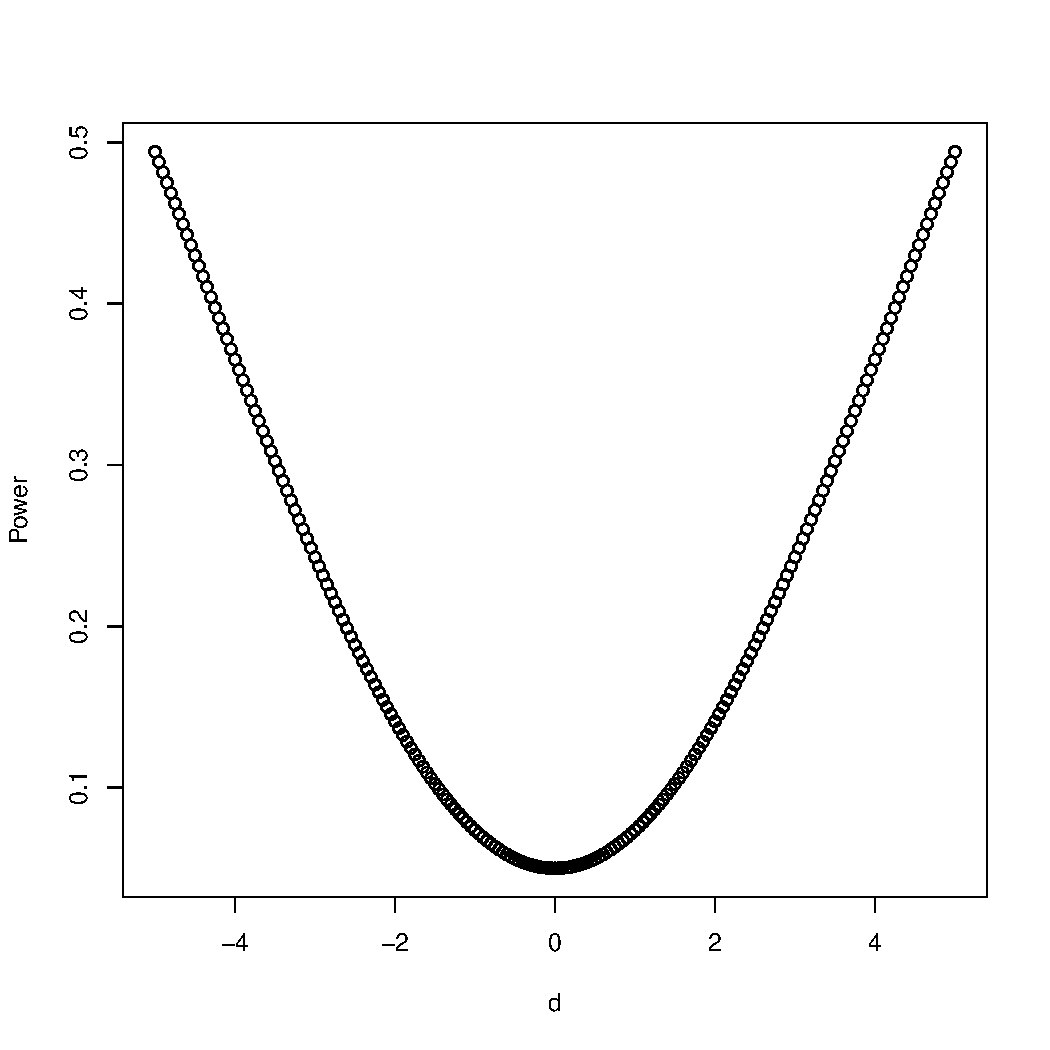
\includegraphics[: :width 0.38\textwidth :]{HW4_3b.pdf}
\caption{Power of an $\alpha$ = 0.05 level test as a function of \emph{d}.}
\end{figure}

\newpage
\section{Appendix: Additional Notes}
\label{sec-4}
\subsection{Useful Theorems}
\label{sec-4-1}


\begin{theorem}
\label{thm:idemchi}
Suppose $\mathbf{Y} \sim MVN_n(\mathbf{\mu}, \mathbf{Sigma})$, $\Sigma$ positive definite. 
Also suppose $\mathbf{A}_{n \times n}$ symmetric and rank($\mathbf{A}$) = $k$.

If $\mathbf{A\Sigma}$ idempotent, $\mathbf{Y'AY} \sim \chi^2_k (\mu'\mathbf{A}\mu)$.

\end{theorem}

\begin{theorem}
Suppose $\mathbf{Y} \sim MVN_n(\mathbf{\mu}, \sigma^2\mathbf{I})$. And the product $\mathbf{BA}=\mathbf{0}$, with A and B of appropriate size.

Then,

\begin{enumerate}[(a)]
\item If $\mathbf{A}$ symmetric, $\mathbf{Y'AY}$ and $\mathbf{BY}$ are independent.
\item If both $\mathbf{B}$ and $\mathbf{A}$ symmetric, $\mathbf{Y'AY}$ and $\mathbf{Y'BY}$ are independent.
\end{enumerate}

\end{theorem}
\subsection{Distributions of interests}
\label{sec-4-2}
\subsubsection{SSE/$\sigma$$^2$}
\label{sec-4-2-1}


Using theorem \ref{thm:idemchi} above, we can show:

$$\frac{SSE}{\sigma^2} = \frac{(\mathbf{Y} -
\hat{\mathbf{Y}})'(\mathbf{Y} - \hat{\mathbf{Y}})}{\sigma^2} \sim
\chi^2_{n-\text{rank}(X)}$$

Rearranging to find confidence limits for $\sigma$ gives:

$$P\left(\sqrt{\frac{SSE}{\mathrm{upper\, \alpha/2\, quantile\, of\,
\chi^2_{n-\mathrm{rank}(X)}}}} < \sigma < \sqrt{\frac{SSE}{\mathrm{upper\, \alpha/2\, quantile\, of\, \chi^2_{n-\mathrm{rank}(X)}}}} \right)
= 1 - \alpha$$
\subsubsection{Estimable functions \textbf{c'$\beta$}}
\label{sec-4-2-2}


For an estimable \textbf{c'$\beta$}, we have:

$$\frac{\widehat{\mathbf{c'\beta}} -
\mathbf{c'\beta}}{\sqrt{MSE}\sqrt{\mathbf{C'(X'X)^{-}C}}} \sim
t_{n-\mathrm{rank}(X)}$$

Note that $MSE = \frac{SSE}{n-\mathrm{rank}(X)}$. Rearranging to find 1 - $\alpha$ confidence limits for \textbf{c'$\beta$},
denoting t$^{\star}$ = the upper $\alpha$/2 quantile of t$_{\mathrm{n-rank(X)}}$, we
have:

$$P\left( \widehat{\mathbf{c'\beta}} -
t^{\star}\sqrt{MSE}\sqrt{\mathbf{C'(X'X)^{-}C}} < \mathbf{c'\beta} <  \widehat{\mathbf{c'\beta}} +
t^{\star}\sqrt{MSE}\sqrt{\mathbf{C'(X'X)^{-}C}} \right) = 1 - \alpha$$
\subsubsection{A t statistic for prediction}
\label{sec-4-2-3}


Consider future observation y$_0$, y$_0$ = \textbf{x$_0$}' $\beta$ + $\epsilon$$_0$ with
$\hat{y}_0 = \mathbf{x_0'\hat{\beta}}$, where $\hat{y_0}$ is computed
from \emph{n} observations and y$_0$ is obtained independently. We find that
$E(y_0 - \hat{y_0}) = 0$ and 


$var(y_0 - \hat{y}_0) = var(\epsilon_0) +
var(\mathbf{x_0'\hat{\beta}}) = \sigma^2[1+
\mathbf{x_0'(X'X)^{-1}x_0}]$, where 
$\widehat{var(y - \hat{y}_0)} = s^22[1+ \mathbf{x_0'(X'X)^{-1}x_0}]$. Because of the independence of \emph{s$^2$}
and \emph{y$_0$} and $\hat{y}_0$, we have the following t statistic:

$$t = \frac{y_0 - \hat{y}_0 - 0}{s\sqrt{1+
\mathbf{x_0'(X'X)^{-1}x_0}}} \sim t(n-\mathrm{rank}(X))$$



Therefore,

$$P = \left[ -t_{\alpha/2,n-rank(X)} \leq \frac{y_0 - \hat{y}_0 - 0}{s\sqrt{1+
\mathbf{x_0'(X'X)^{-1}x_0}}} \leq t_{alpha/2,n-rank(X)}\right] = 1 -
\alpha$$

Re-arranging in terms of $\mathbf{x_0'\hat{\beta}} = \hat{y}_0$ gives:

$$\mathbf{x_0'\hat{\beta}} \pm t_{\alpha/2,n-rank(X)}s\sqrt{1+
\mathbf{x_0'(X'X)^{-1}x_0}}.$$
\subsection{General Linear Hypothesis Test}
\label{sec-4-3}

\emph{The general linear hypothesis test} is the following F test for
\emph{H$_0$} : \textbf{C$\beta$} = \textbf{0} verus \emph{H$_1$} : \textbf{C$\beta$} $\neq$ \textbf{0}, given \textbf{y}
$\sim$ N$_n$(\textbf{X$\beta$},$\sigma$$^2$ \textbf{I}), \textbf{C} \emph{q} x (/k/+1), rank(\textbf{C}) = q, with SSH = the sum of squares due to
the hypothesis or due to \textbf{C$\beta$}. Note that 

\(\frac{SSH}{\sigma^2} = \frac{(\mathbf{C\hat{\beta}})'[\mathbf{C(X'X)^{-1}C}']^{-1}\mathbf{C\hat{\beta}}}{\sigma^2}
\sim
\chi^2(q,\frac{(\mathbf{C\beta})'[\mathbf{C(X'X)^{-1}C}']^{-1}\mathbf{C\beta}}{2\sigma^2})\)

\noindent and

\(\frac{SSE}{\sigma^2} = \frac{\mathbf{y}'[\mathbf{I} -
\mathbf{X(X'X)^{-1}X}']\mathbf{y}}{\sigma^2} \sim \chi^2(n-rank(X)).\)

Taking the ratio gives us our test statistic:
$$F = \frac{SSH/q}{SSE/(n-rank(X))}$$

\begin{itemize}
\item If \emph{H$_0$} : \textbf{C$\beta$} = \textbf{0} is false, F $\sim$ F(q,n-rank(X),$\lambda$), where
  $\lambda =
  \frac{(\mathbf{C\beta})'[\mathbf{C(X'X)^{-1}C}']^{-1}\mathbf{C\beta}}{2\sigma^2})$.
\item Notice that if \textbf{C$\beta$} = \textbf{0} is true, $\lambda$ defined above = 0, giving F
  $\sim$ F(q, n-rank(X)).
\end{itemize}
\section{Appendix: Tangled R code}
\label{sec-5}


\lstinputlisting{DabbishHW4c.R}

\end{document}
